\chapter{Presión, energía libre y fluctuaciones de la energía}

\lectureoverview{Derivamos la presión a partir de la función de partición sin suponer un modelo cinético de moléculas que chocan contra una pared. Un lema geométrico transforma una derivada adiabática en derivadas a temperatura constante; la energía libre de Helmholtz proporciona el vínculo con \(\log Z\), y la ley del gas ideal se obtiene como primera aplicación. Después usamos la misma función de partición para derivar la fluctuación de energía en equilibrio y su relación con la capacidad calorífica.}

\section{Dejemos que las matemáticas pongan a prueba la intuición}

La termodinámica tiene una reputación peculiar. Su cálculo es elemental, pero puede ser sorprendentemente sutil elegir qué derivar y qué mantener fijo. Nuestro problema es deliberadamente acotado: calcular la presión de un gas ideal. Sin embargo, el procedimiento para obtener la respuesta pretende ser lo bastante general como para aplicarse a sistemas en los que el conocido modelo molecular deja de ser fiable.

La explicación cinética es fácil de contar. Las moléculas chocan contra una pared e invierten la componente normal de su cantidad de movimiento. La cantidad de movimiento transferida por unidad de tiempo da la fuerza, y la fuerza por unidad de área da la presión. Ya sabemos que la energía cinética media por molécula en tres dimensiones es \begin{equation}
 \left\langle \frac{p^2}{2m}\right\rangle=\frac{3}{2}T
 \qquad (k_B=1).
 \label{eq:sm5-mean-kinetic-energy}
\end{equation} Con una distribución isotrópica de velocidades se pueden estimar la frecuencia de colisión, la transferencia de cantidad de movimiento en cada choque y la presión resultante.

Pero la propia pared parece romper la isotropía. ¿Por qué habrían de tener las moléculas muy próximas al límite la misma distribución de velocidades y direcciones que las moléculas en el interior? En equilibrio la tienen, con la precisión pertinente aquí, pero esa conclusión debería derivarse de la mecánica estadística en vez de introducirse subrepticiamente en el cálculo como una intuición. Las colisiones entre moléculas hacen que el argumento cinético sea aún menos transparente. El gas no interactuante es fácil precisamente porque constituye un sistema excepcionalmente sencillo.

En física hay ocasiones en que el procedimiento más seguro consiste en dejar de lado momentáneamente el modelo intuitivo y seguir las matemáticas. Se identifica la cantidad que se busca, se manipulan las relaciones generales y se espera hasta que aparezca una fórmula reconocible. La intuición vuelve al final, pero entonces son las matemáticas las que ponen a prueba la intuición, y no al revés. El atractivo de la termodinámica reside en las relaciones sorprendentes que surgen de este procedimiento.

La relación buscada es una ecuación de estado: \begin{equation}
 P=P(T,V,N),
 \label{eq:sm5-equation-of-state-target}
\end{equation} donde \(N\) es la cantidad de sustancia, \(T\) la temperatura y \(V\) el volumen. Una derivación satisfactoria debería seguir teniendo sentido cuando las partículas interactúan o cuando la sustancia es un líquido, un plasma o un sólido. Solo el cálculo final de la función de partición se especializará al caso del gas ideal.

\section{Entropía y energía libre de Helmholtz}

Empecemos por recordar las fórmulas del ensamble canónico que necesitaremos más adelante. Para microestados etiquetados por \(i\): \begin{equation}
 \begin{aligned}
 S&=-\sum_i p_i\log p_i,\\
 p_i&=\frac{e^{-\beta E_i}}{Z},\\
 Z&=\sum_i e^{-\beta E_i}.
 \end{aligned}
 \label{eq:sm5-canonical-definitions}
\end{equation} El logaritmo de la probabilidad es \begin{equation}
 \log p_i=-\beta E_i-\log Z.
 \label{eq:sm5-log-probability}
\end{equation} Al sustituirlo en la expresión de la entropía se obtiene \begin{align}
 S
 &=-\sum_i p_i\log p_i \notag\\
 &=\beta\sum_i p_iE_i+\log Z\sum_i p_i \notag\\
 &=\beta E+\log Z.
 \label{eq:sm5-entropy-log-z}
\end{align} Aquí \(E=\sum_i p_iE_i\) es la energía media.

\begin{classroomqa}\audiencequestion{¿Por qué el segundo término da solo \(\log Z\) y no el número de estados multiplicado por \(\log Z\)?}\lecturerresponse{El coeficiente que se suma es \(p_i\), no \(1\). La normalización da \(\sum_i p_i=1\). Equivalentemente, el numerador \(\sum_i e^{-\beta E_i}=Z\) cancela el \(Z\) del denominador. El número de estados no interviene en este paso. \lecturetimestamp{00:14:25--00:14:55}}\end{classroomqa}

En las unidades de energía que usaremos durante la mayor parte de la clase, \(\beta=1/T\). Al multiplicar \eqref{eq:sm5-entropy-log-z} por \(T\) y reordenar, se obtiene \begin{equation}
 E-TS=-T\log Z.
 \label{eq:sm5-helmholtz-identity}
\end{equation} La combinación del lado izquierdo aparece tan a menudo que merece un nombre: \begin{equation}
 A\equiv E-TS,
 \qquad
 A=-T\log Z.
 \label{eq:sm5-helmholtz-definition}
\end{equation} Es la energía libre de Helmholtz. Por ahora, el nombre importa menos que la propia identidad; la necesitaremos para expresar la presión como una derivada de la función de partición.

\begin{figure}[t]\centering
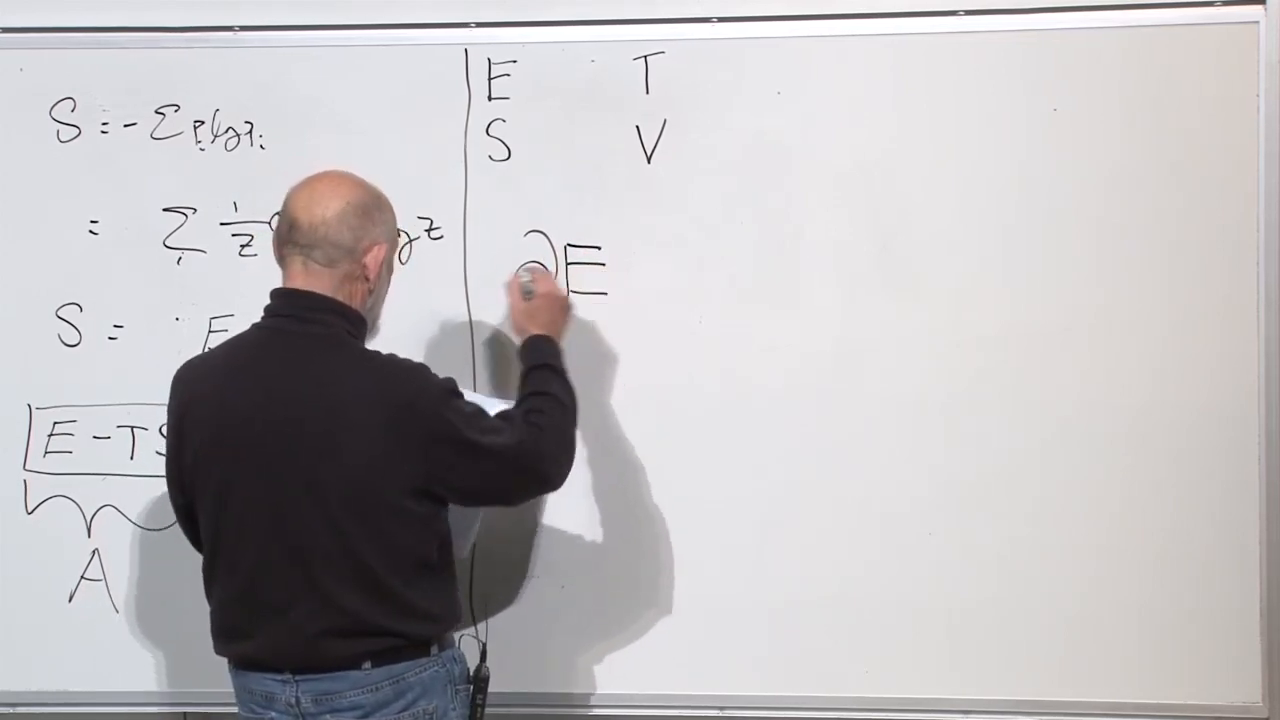
\includegraphics[width=0.90\textwidth]{lecture_05_figure_03.png}\caption{La relación canónica para la entropía reordenada como \(A=E-TS=-T\log Z\).}\lectureframe{00:16:50}\end{figure}

\section{Parámetros de control y sus respuestas}

Un parámetro de control es una magnitud macroscópica que un experimentador puede modificar desde el exterior. Al mover un pistón se cambia el volumen sin manipular moléculas individuales. Los campos eléctricos y magnéticos aplicados son otros ejemplos. En un ensamble más general también se puede permitir que cambie el número de partículas.

Las variables termodinámicas se presentan naturalmente en pares conjugados. En el problema actual, el volumen es el parámetro de control y la presión su respuesta. Cambiamos \(V\); la presión indica cómo se opone energéticamente el sistema a ese cambio. Más adelante, la derivada de la energía precisará esta relación.

\begin{classroomqa}\audiencequestion{¿Puede considerarse la presión misma como parámetro de control?}\lecturerresponse{Se puede diseñar un experimento que mantenga fija la presión externa, pero en el montaje que usamos aquí la posición del pistón fija el volumen y la presión interna es la respuesta. La presión y el volumen son variables conjugadas; cuál de ellas se controla depende del ensamble y del aparato. \lecturetimestamp{00:19:22--00:20:01}}\end{classroomqa}

\begin{classroomqa}\audiencequestion{¿Se supone que todas las moléculas son idénticas o el argumento se limita a un gas?}\lecturerresponse{El argumento termodinámico no requiere ninguna de esas restricciones. El cilindro puede contener varias especies, un líquido o incluso un sólido sometido a compresión. La función de partición del gas ideal será solo una aplicación particular, después de establecer la fórmula general de la presión. \lecturetimestamp{00:20:02--00:20:39}}\end{classroomqa}

\begin{classroomqa}\audiencequestion{¿Se podría cambiar la cantidad de sustancia mediante otra operación externa?}\lecturerresponse{Sí. El número de partículas es otro posible parámetro de control. Si se trata dinámicamente, aparece su propia variable conjugada: el potencial químico. Para el cálculo de hoy, \(N\) permanece fijo. \lecturetimestamp{00:20:39--00:20:57}}\end{classroomqa}

\begin{classroomqa}\audiencequestion{¿Pueden coexistir en equilibrio el agua líquida y el vapor?}\lecturerresponse{Pueden hacerlo a la temperatura y presión de coexistencia. La gravedad puede situar el líquido debajo del vapor y, aun así, ambas fases pueden compartir una misma temperatura y permanecer en equilibrio térmico. Se aplica el mismo marco general de la mecánica estadística. \lecturetimestamp{00:20:59--00:21:36}}\end{classroomqa}

Para el siguiente argumento, consideremos la energía y la entropía como funciones dependientes de dos variables que se pueden ajustar independientemente: \begin{equation}
 E=E(T,V),
 \qquad
 S=S(T,V).
 \label{eq:sm5-dependent-functions}
\end{equation} La temperatura y el volumen proporcionan coordenadas en el espacio de estados termodinámicos. La energía y la entropía asignan valores a cada punto de equilibrio de ese espacio.

\section{La derivada a entropía constante}

La derivada que necesitamos en última instancia es poco habitual: \[
 \left(\frac{\partial E}{\partial V}\right)_S.
\] Aunque \(T\) y \(V\) son las coordenadas independientes, esta derivada pide variar \(V\) mientras se impone que la función dependiente \(S(T,V)\) permanezca constante. Es una derivada a lo largo de una curva en el plano \((T,V)\), no a lo largo de un eje de coordenadas.

\begin{classroomqa}\audiencequestion{¿Cómo pueden ser independientes \(T\) y \(V\) si más adelante se usa una derivada \(dT/dV\)?}\lecturerresponse{Son independientes en el espacio de estados completo. Al imponer la restricción \(S(T,V)=\mathrm{constant}\), los estados permitidos quedan sobre una curva unidimensional. A lo largo de esa curva, \(T\) pasa a ser función de \(V\) y su pendiente \(dT/dV\) está bien definida. \lecturetimestamp{01:01:18--01:02:09}}\end{classroomqa}

\begin{lemma}Si \(E(T,V)\) y \(S(T,V)\) son diferenciables, entonces, dondequiera que \((\partial S/\partial T)_V\neq0\): \begin{equation}
 \left(\frac{\partial E}{\partial V}\right)_S
 =
 \left(\frac{\partial E}{\partial V}\right)_T
 -
 \left(\frac{\partial E}{\partial S}\right)_V
 \left(\frac{\partial S}{\partial V}\right)_T.
 \label{eq:sm5-calculus-lemma}
\end{equation}\end{lemma}

\begin{proof}Para un desplazamiento infinitesimal arbitrario: \begin{equation}
 dE=
 \left(\frac{\partial E}{\partial V}\right)_T dV
 +
 \left(\frac{\partial E}{\partial T}\right)_V dT.
 \label{eq:sm5-total-differential-e}
\end{equation} A \(V\) constante, la regla de la cadena permite usar \(S\) como variable intermedia: \begin{equation}
 \left(\frac{\partial E}{\partial T}\right)_V
 =
 \left(\frac{\partial E}{\partial S}\right)_V
 \left(\frac{\partial S}{\partial T}\right)_V.
 \label{eq:sm5-chain-rule-e-s-t}
\end{equation}

Restringimos ahora el desplazamiento a una curva en la que \(S\) es constante. A lo largo de esa curva, \begin{equation}
 0=dS=
 \left(\frac{\partial S}{\partial V}\right)_T dV
 +
 \left(\frac{\partial S}{\partial T}\right)_V dT.
 \label{eq:sm5-constant-entropy-differential}
\end{equation} Despejando la pendiente de la curva se obtiene \begin{equation}
 \left(\frac{dT}{dV}\right)_S
 =
 -
 \frac{\left(\frac{\partial S}{\partial V}\right)_T}
 {\left(\frac{\partial S}{\partial T}\right)_V}.
 \label{eq:sm5-entropy-contour-slope}
\end{equation} Dividimos \eqref{eq:sm5-total-differential-e} por \(dV\), usamos \eqref{eq:sm5-chain-rule-e-s-t} e insertamos \eqref{eq:sm5-entropy-contour-slope}: \begin{align}
 \left(\frac{\partial E}{\partial V}\right)_S
 &=
 \left(\frac{\partial E}{\partial V}\right)_T
 +
 \left(\frac{\partial E}{\partial S}\right)_V
 \left(\frac{\partial S}{\partial T}\right)_V
 \left(\frac{dT}{dV}\right)_S \notag\\
 &=
 \left(\frac{\partial E}{\partial V}\right)_T
 -
 \left(\frac{\partial E}{\partial S}\right)_V
 \left(\frac{\partial S}{\partial V}\right)_T.
\end{align} El factor \((\partial S/\partial T)_V\) se ha cancelado, lo que demuestra el resultado. \end{proof}

\begin{figure}[t]\centering
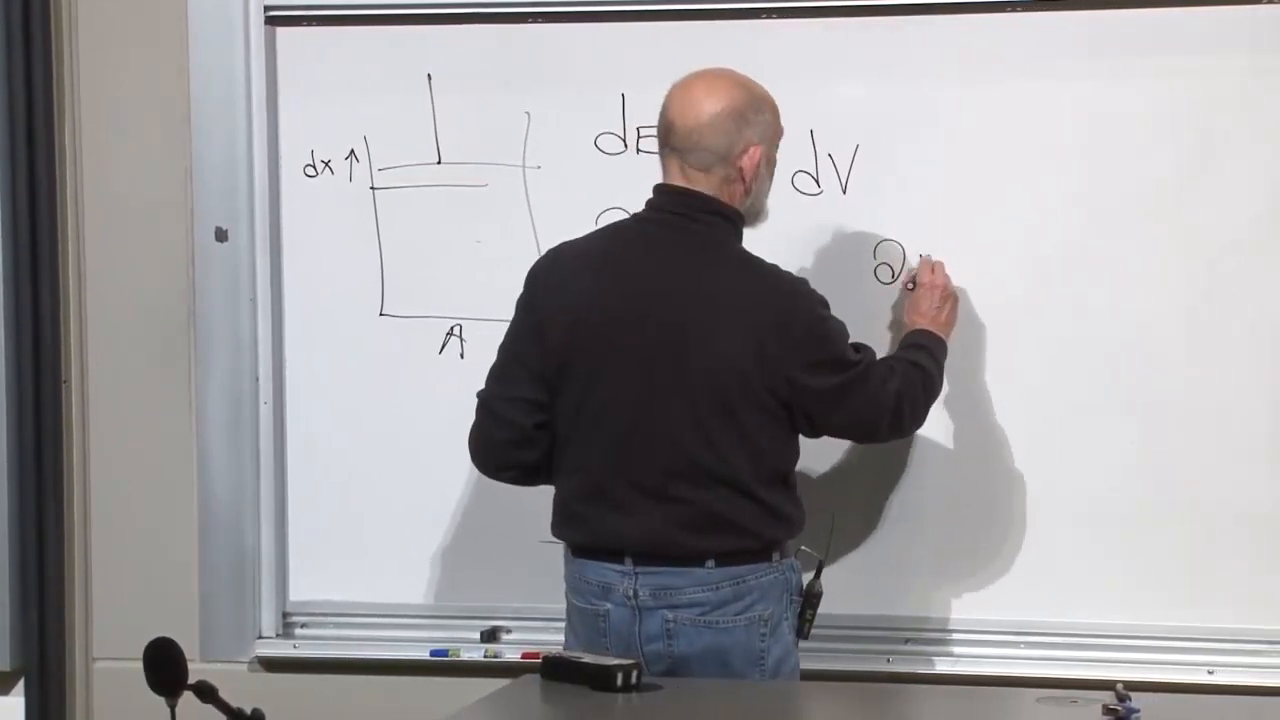
\includegraphics[width=0.90\textwidth]{lecture_05_figure_04.png}\caption{Cálculo sobre la curva de entropía constante, en el punto de cancelación que completa el lema sobre derivadas.}\lectureframe{00:36:10}\end{figure}

La interpretación geométrica no es un mero adorno. Explica por qué una derivada a \(S\) constante que parece extraña se puede calcular mediante derivadas parciales ordinarias en las coordenadas independientes \(T\) y \(V\). Escribir \(\delta E/\delta V\) durante la construcción sirve para recordar que los símbolos representan cocientes de cambios pequeños a lo largo de una trayectoria especificada.

\begin{classroomqa}\audiencequestion{¿El desarrollo de \(dE\) es simplemente la definición habitual de las derivadas parciales?}\lecturerresponse{Sí. En el diferencial total no hay nada especial. El único ingrediente adicional es la restricción posterior a la curva \(dS=0\), que determina la relación entre \(dT\) y \(dV\). \lecturetimestamp{00:29:26--00:29:32}}\end{classroomqa}

\begin{classroomqa}\audiencequestion{¿La cancelación requiere que \((\partial S/\partial T)_V\) sea distinto de cero?}\lecturerresponse{Sí. Para un sistema estable ordinario, \[
 \left(\frac{\partial S}{\partial T}\right)_V
 =\frac{C_V}{T}>0,
\] así que la división está justificada. Los puntos excepcionales requieren un análisis aparte. Con el Hamiltoniano fijo, elevar la temperatura ensancha la distribución canónica de energía y normalmente aumenta la entropía; bajar la temperatura la estrecha. Esta es la orientación físicamente correcta del argumento de monotonía. \lecturetimestamp{00:36:50--00:37:47}}\end{classroomqa}

\section{Trabajo del pistón y condición adiabática}

Ahora daremos un significado físico a la derivada. Consideremos un pistón de área transversal \(\mathcal A\). Si se desplaza hacia fuera una distancia \(dx\), entonces \begin{equation}
 dV=\mathcal A\,dx.
 \label{eq:sm5-piston-volume}
\end{equation} El gas ejerce sobre el pistón una fuerza \(P\mathcal A\), de modo que el trabajo realizado por el gas es \begin{equation}
 \delta W_{\mathrm{by}}=P\mathcal A\,dx=P\,dV.
 \label{eq:sm5-piston-work}
\end{equation} Si no entra calor en el gas, la conservación de la energía da \begin{equation}
 dE=-P\,dV.
 \label{eq:sm5-adiabatic-work}
\end{equation} El signo tiene un significado físico: durante la expansión, el gas eleva el pistón o lo acelera, y su propia energía disminuye.

\begin{figure}[t]\centering
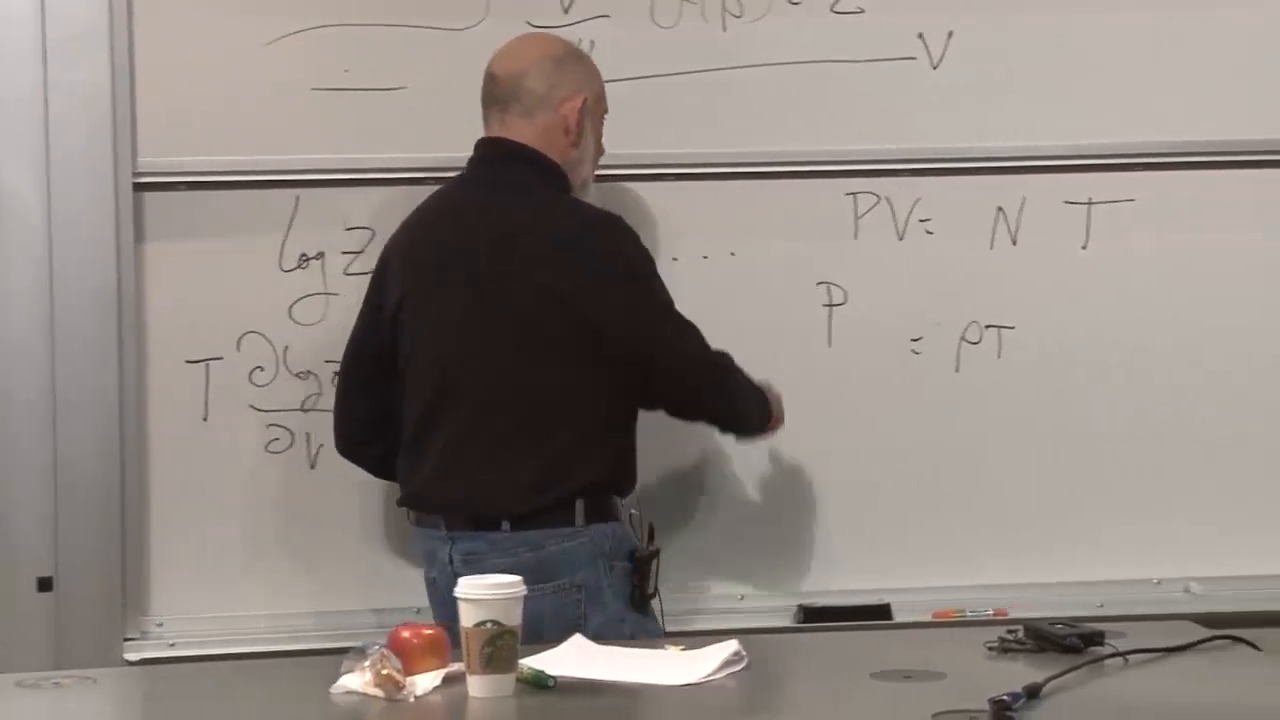
\includegraphics[width=0.90\textwidth]{lecture_05_figure_05.png}\caption{Geometría del pistón y relación de trabajo resultante \(dE=-P\,dV\).}\lectureframe{00:43:10}\end{figure}

Hay dos condiciones esenciales. El pistón debe moverse con suficiente lentitud para que el sistema permanezca tan cerca del equilibrio como se quiera, y las paredes deben estar aisladas para que no se suministre energía en forma de calor. Una tracción rápida puede ser tan breve que ninguna molécula alcance el pistón, que se aleja, durante el movimiento. Una compresión rápida genera ondas de choque. Ninguno de estos procesos se representa mediante una sucesión de estados de equilibrio.

A veces se usa la palabra \emph{adiabático} para indicar ausencia de transferencia de calor y otras veces para indicar un cambio lento. En el proceso reversible que necesitamos intervienen ambas ideas: el cambio es cuasiestático y térmicamente aislado. En esas condiciones, también es isentrópico.

\begin{classroomqa}\audiencequestion{¿Por qué un cambio adiabático mantiene constante la entropía?}\lecturerresponse{Consideremos el sistema desde el punto de vista de la mecánica cuántica. Sus niveles de energía de muchos cuerpos dependen del volumen. Cuando \(V\) cambia lentamente, el teorema adiabático lleva cada nivel ocupado de manera continua a su nivel sucesor, sin transiciones entre las etiquetas de los niveles. Las energías \(E_i(V)\) cambian, pero las probabilidades de ocupación \(p_i\) permanecen fijas. Como \(S=-\sum_i p_i\log p_i\) depende de esas probabilidades, la entropía permanece constante. El intercambio de calor o el movimiento irreversible invalidarían esta conclusión. \lecturetimestamp{00:43:37--00:49:15}}\end{classroomqa}

\begin{figure}[t]\centering
\includegraphics[width=0.90\textwidth]{lecture_05_figure_06.png}\caption{Niveles de energía de muchos cuerpos que varían con el volumen mientras sus probabilidades de ocupación conservan las etiquetas de los niveles.}\lectureframe{00:48:50}\end{figure}

La ecuación \eqref{eq:sm5-adiabatic-work}, evaluada a lo largo de esta trayectoria de entropía constante, identifica la presión como \begin{equation}
 P=-\left(\frac{\partial E}{\partial V}\right)_S.
 \label{eq:sm5-pressure-fixed-entropy}
\end{equation} Esta es la relación conjugada entre presión y volumen.

\begin{classroomqa}\audiencequestion{¿Qué ocurre si el pistón se mueve rápidamente?}\lecturerresponse{El sistema deja de estar en equilibrio y su dinámica detallada pasa a ser relevante. Una compresión brusca genera una onda de choque. En una expansión libre ideal, el pistón puede alejarse antes de que ninguna molécula choque contra él, por lo que no se realiza trabajo y la energía permanece constante aunque cambie el volumen. Después, el gas se relaja hasta alcanzar el equilibrio y su entropía aumenta. Estos procesos no pueden describirse mediante la única derivada de equilibrio en \eqref{eq:sm5-pressure-fixed-entropy}. \lecturetimestamp{00:58:30--01:01:15}}\end{classroomqa}

\begin{classroomqa}\audiencequestion{¿Qué condición cuantitativa determina si un cambio es lento?}\lecturerresponse{El tiempo de variación externa debe ser largo en comparación con los tiempos de relajación internos pertinentes. En un gas, durante el cambio macroscópico deberían producirse muchas colisiones moleculares y muchos choques contra las paredes. La escala temporal precisa depende del material y la geometría, mientras que el límite cuasiestático es general. \lecturetimestamp{01:02:09--01:03:20}}\end{classroomqa}

\section{De la energía adiabática a la función de partición}

La fórmula física \eqref{eq:sm5-pressure-fixed-entropy} todavía no es la más fácil de calcular. La mecánica estadística canónica proporciona naturalmente funciones de la temperatura, porque \(T\) aparece directamente en el factor de Boltzmann. El lema de cálculo transforma la incómoda derivada a entropía constante en una forma que facilita el cálculo: \begin{align}
 P
 &=
 -\left(\frac{\partial E}{\partial V}\right)_T
 +
 \left(\frac{\partial E}{\partial S}\right)_V
 \left(\frac{\partial S}{\partial V}\right)_T.
 \label{eq:sm5-pressure-lemma-substitution}
\end{align} A volumen constante, la primera ley da \(dE=T\,dS\) y, por tanto, \begin{equation}
 \left(\frac{\partial E}{\partial S}\right)_V=T.
 \label{eq:sm5-e-s-temperature}
\end{equation} Así pues: \begin{equation}
 P=
 -\left(\frac{\partial E}{\partial V}\right)_T
 +
 T\left(\frac{\partial S}{\partial V}\right)_T.
 \label{eq:sm5-pressure-fixed-temperature-pieces}
\end{equation}

\begin{classroomqa}\audiencequestion{¿De dónde viene el signo menos de la fórmula de la presión?}\lecturerresponse{Se origina en el trabajo realizado por el gas: \(dE=-P\,dV\) durante la expansión adiabática. El lema de cálculo tiene por sí mismo un signo menos entre sus dos términos; el signo menos global de \(P=-(\partial E/\partial V)_S\) cambia el signo de ambos, y se obtiene \eqref{eq:sm5-pressure-fixed-temperature-pieces}. \lecturetimestamp{00:52:40--00:53:14}}\end{classroomqa}

Como \(T\) se mantiene fijo en ambas derivadas, \begin{align}
 P
 &=
 -\left(\frac{\partial}{\partial V}(E-TS)\right)_T \notag\\
 &=
 -\left(\frac{\partial A}{\partial V}\right)_T.
 \label{eq:sm5-pressure-free-energy}
\end{align} Por último, sustituimos \(A=-T\log Z\): \begin{equation}
 \boxed{
 P=
 T\left(\frac{\partial\log Z}{\partial V}\right)_T
 }.
 \label{eq:sm5-pressure-log-z}
\end{equation}

\begin{figure}[t]\centering
\includegraphics[width=0.90\textwidth]{lecture_05_figure_07.png}\caption{Compresión del argumento a temperatura constante: \(P=-(\partial A/\partial V)_T
=T(\partial\log Z/\partial V)_T\).}\lectureframe{00:55:55}\end{figure}

Nada en \eqref{eq:sm5-pressure-log-z} presupone que el gas sea ideal. Si se puede calcular la función de partición de un fluido interactuante, un plasma o un sólido, la misma derivada da su presión. En términos más generales, cada parámetro de control externo tiene una respuesta conjugada que se obtiene derivando un potencial termodinámico apropiado. La función de partición reúne muchas de esas respuestas: derivar \(\log Z\) con respecto a \(\beta\) da la energía, mientras que derivarla con respecto al volumen da la presión.

\section{La ecuación de estado del gas ideal}

Solo ahora nos restringimos a \(N\) partículas no interactuantes. Conservando la normalización clásica del espacio de fases, \begin{equation}
 Z_N=
 \frac{1}{N!h^{3N}}
 \int d^{3N}q\,d^{3N}p\,
 \exp\!\left[
 -\beta\sum_{a=1}^{N}\frac{\mathbf p_a^2}{2m}
 \right].
 \label{eq:sm5-ideal-gas-partition-integral}
\end{equation} Hay \(3N\) coordenadas de posición y \(3N\) coordenadas de momento. El Hamiltoniano no depende de la posición, por lo que cada partícula aporta un factor igual al volumen del recipiente: \begin{equation}
 Z_N=
 \frac{V^N}{N!h^{3N}}I_p(\beta),
 \label{eq:sm5-ideal-gas-factorization}
\end{equation} donde la integral de momento completa \(I_p(\beta)\) no depende de \(V\).

\begin{classroomqa}\audiencequestion{¿Por qué hay \(3N\) integrales de posición y \(3N\) integrales de momento?}\lecturerresponse{Cada una de las \(N\) partículas tiene tres coordenadas espaciales y tres componentes de momento conjugadas. El número es \(3N\) en cada mitad del espacio de fases, no \(N\) partículas más otras \(3N\) partículas. \lecturetimestamp{01:04:19--01:04:28}}\end{classroomqa}

Al tomar el logaritmo se separa la dependencia del volumen: \begin{equation}
 \log Z_N
 =
 N\log V-\log N!-3N\log h+\log I_p(\beta).
 \label{eq:sm5-log-ideal-gas-partition}
\end{equation} Los factores \(1/N!\), \(h^{-3N}\) y \(I_p(\beta)\) son todos independientes del volumen. Importan para la entropía absoluta y otras cuestiones, pero no para esta derivada concreta. Por tanto, \begin{equation}
 \left(\frac{\partial\log Z_N}{\partial V}\right)_T
 =\frac{N}{V}.
 \label{eq:sm5-log-z-volume-derivative}
\end{equation} La ecuación \eqref{eq:sm5-pressure-log-z} da inmediatamente \begin{equation}
 P=\frac{NT}{V},
 \qquad
 \boxed{PV=NT}.
 \label{eq:sm5-ideal-gas-law}
\end{equation}

\begin{classroomqa}\audiencequestion{¿Sigue \(N\) contando las réplicas usadas para derivar la distribución de Boltzmann?}\lecturerresponse{No. La construcción con réplicas fue un recurso de conteo en la derivación anterior y ya no interviene. Aquí, \(N\) es el número de partículas físicas de esta muestra de gas. \lecturetimestamp{01:07:38--01:08:05}}\end{classroomqa}

Al definir la densidad numérica \begin{equation}
 \rho=\frac{N}{V}
 \label{eq:sm5-number-density}
\end{equation} se obtiene la forma equivalente \begin{equation}
 P=\rho T.
 \label{eq:sm5-density-equation-of-state}
\end{equation}

\begin{classroomqa}\audiencequestion{¿Se obtiene la expresión en términos de la densidad dividiendo por \(N\) o por \(V\)?}\lecturerresponse{Dividimos \(PV=NT\) por \(V\): \(P=(N/V)T=\rho T\). Aquí \(\rho\) es la densidad numérica, no la densidad de masa. \lecturetimestamp{01:08:45--01:09:16}}\end{classroomqa}

\begin{figure}[t]\centering
\includegraphics[width=0.90\textwidth]{lecture_05_figure_08.png}\caption{La derivada respecto al volumen de \(\log Z\) y la ecuación de estado resultante del gas ideal \(PV=NT\), o bien \(P=\rho T\).}\lectureframe{01:09:25}\end{figure}

Al recuperar la temperatura de laboratorio \(T_K\): \begin{equation}
 PV=Nk_BT_K.
 \label{eq:sm5-ideal-gas-law-laboratory}
\end{equation} El resultado conocido concuerda con la intuición cinética, pero su derivación se apoya ahora en un marco que va mucho más allá del gas libre.

\section{Un segundo fruto: las fluctuaciones de equilibrio}

El cálculo de la presión está completo, pero queda una pregunta que habíamos prometido responder: ¿qué más se puede extraer de la función de partición? Consideremos un sistema en contacto térmico con un baño de calor. Su energía no es fija. La energía entra y sale, por lo que las mediciones repetidas fluctúan alrededor de la media canónica.

\begin{classroomqa}\audiencequestion{¿Podemos calcular ahora las fluctuaciones prometidas?}\lecturerresponse{Sí. El tiempo adicional permite una segunda demostración del mismo principio: las derivadas de \(Z\) codifican información termodinámica medible. \lecturetimestamp{01:10:37--01:10:50}}\end{classroomqa}

\subsection{Varianza y desviación estándar}

Para una variable aleatoria \(x\) con \(\langle x\rangle=0\), una medida de la amplitud de la distribución es \(\langle x^2\rangle\). Para una distribución general, desplazamos la variable restándole su media: \begin{equation}
 \delta x=x-\langle x\rangle.
 \label{eq:sm5-centered-variable}
\end{equation} Su media es cero: \begin{equation}
 \langle\delta x\rangle
 =
 \langle x\rangle-\langle x\rangle=0,
 \label{eq:sm5-centered-mean}
\end{equation} y su media cuadrática es \begin{align}
 (\Delta x)^2
 &\equiv
 \left\langle\left(x-\langle x\rangle\right)^2\right\rangle \notag\\
 &=
 \langle x^2\rangle
 -2\langle x\rangle^2
 +\langle x\rangle^2 \notag\\
 &=
 \langle x^2\rangle-\langle x\rangle^2.
 \label{eq:sm5-variance}
\end{align} Esta es la varianza. Su raíz cuadrada positiva \(\Delta x\) es la desviación estándar.

\begin{classroomqa}\audiencequestion{¿Por qué el promedio de \(x-\langle x\rangle\) es exactamente cero?}\lecturerresponse{Los promedios son lineales, y \(\langle x\rangle\) ya es un número. Por tanto, \(\langle x-\langle x\rangle\rangle
=\langle x\rangle-\langle x\rangle=0\). \lecturetimestamp{01:14:02--01:14:22}}\end{classroomqa}

\begin{classroomqa}\audiencequestion{¿Qué diferencia hay entre fluctuación cuadrática, varianza, amplitud cuadrática media y desviación estándar?}\lecturerresponse{La varianza es \((\Delta x)^2=\langle x^2\rangle-\langle x\rangle^2\). La desviación estándar es su raíz cuadrada, \(\Delta x\). Para una variable de media cero, la desviación estándar también es su valor cuadrático medio. \lecturetimestamp{01:16:39--01:18:38}}\end{classroomqa}

\begin{figure}[t]\centering
\includegraphics[width=0.90\textwidth]{lecture_05_figure_09.png}\caption{La variable centrada y el desarrollo que da lugar a \((\Delta x)^2=\langle x^2\rangle-\langle x\rangle^2\).}\lectureframe{01:17:20}\end{figure}

\subsection{Momentos de energía a partir de la función de partición}

Para el ensamble canónico, \begin{align}
 \langle E\rangle
 &=
 \frac{1}{Z}\sum_i E_i e^{-\beta E_i} \notag\\
 &=
 -\frac{1}{Z}\frac{\partial Z}{\partial\beta}
 =
 -\frac{\partial\log Z}{\partial\beta}.
 \label{eq:sm5-mean-energy-from-z}
\end{align} La multiplicación por un factor \(E_i\) se obtiene mediante una derivada negativa respecto de \(\beta\). Una segunda derivada genera \(E_i^2\): \begin{equation}
 \langle E^2\rangle
 =
 \frac{1}{Z}\sum_i E_i^2e^{-\beta E_i}
 =
 \frac{1}{Z}\frac{\partial^2 Z}{\partial\beta^2}.
 \label{eq:sm5-second-energy-moment}
\end{equation} En consecuencia, la varianza de la energía es \begin{align}
 (\Delta E)^2
 &=
 \langle E^2\rangle-\langle E\rangle^2 \notag\\
 &=
 \frac{1}{Z}\frac{\partial^2Z}{\partial\beta^2}
 -
 \frac{1}{Z^2}
 \left(\frac{\partial Z}{\partial\beta}\right)^2 \notag\\
 &=
 \frac{\partial^2\log Z}{\partial\beta^2}
 =
 -\frac{\partial\langle E\rangle}{\partial\beta}.
 \label{eq:sm5-energy-variance-beta}
\end{align} Una vez más, un observable que parece complicado se convierte en una derivada de \(\log Z\).

\begin{figure}[t]\centering
\includegraphics[width=0.90\textwidth]{lecture_05_figure_10.png}\caption{La segunda derivada respecto de \(\beta\) de \(\log Z\), identificada con la varianza de la energía.}\lectureframe{01:29:00}\end{figure}

\subsection{Capacidad calorífica y magnitud de las fluctuaciones}

En las unidades usadas en la clase, \(T=1/\beta\), de modo que \begin{equation}
 -\frac{\partial}{\partial\beta}
 =
 T^2\frac{\partial}{\partial T}.
 \label{eq:sm5-beta-temperature-derivative}
\end{equation} A volumen constante, definimos la capacidad calorífica de la muestra completa como \begin{equation}
 C_V\equiv
 \left(\frac{\partial\langle E\rangle}{\partial T}\right)_V.
 \label{eq:sm5-heat-capacity}
\end{equation} La ecuación \eqref{eq:sm5-energy-variance-beta} queda \begin{equation}
 \boxed{(\Delta E)^2=T^2C_V}
 \qquad (k_B=1).
 \label{eq:sm5-energy-fluctuation-lecture-units}
\end{equation} Para la temperatura de laboratorio \(T_K\), donde \(\beta=(k_BT_K)^{-1}\), \begin{equation}
 \boxed{(\Delta E)^2=k_BT_K^2C_V}.
 \label{eq:sm5-energy-fluctuation-laboratory}
\end{equation}

\begin{figure}[t]\centering
\includegraphics[width=0.90\textwidth]{lecture_05_figure_11.png}\caption{Conversión de la derivada respecto de \(\beta\) a la capacidad calorífica a volumen constante, incluido el factor \(k_B\) restituido.}\lectureframe{01:31:10}\end{figure}

\begin{classroomqa}\audiencequestion{¿La derivada debe especificar volumen constante en vez de presión constante?}\lecturerresponse{Sí. Esta derivación canónica mantiene fijos los parámetros de control externos del Hamiltoniano, incluido \(V\). La magnitud resultante es \(C_V\). En un ensamble a presión constante, el volumen y el trabajo pueden fluctuar, y se necesita el potencial termodinámico correspondiente; no se puede sustituir simplemente \(C_V\) por \(C_P\) en \eqref{eq:sm5-energy-fluctuation-laboratory}. \lecturetimestamp{01:29:01--01:29:28; 01:32:50--01:33:21}}\end{classroomqa}

\begin{classroomqa}\audiencequestion{¿Es \(C_V\) una constante del material?}\lecturerresponse{En general, no. Puede depender de la temperatura, el volumen, la fase y la composición. Además, \(C_V\) es aquí la capacidad calorífica de la muestra completa y es extensiva. El calor específico se obtiene solo al dividir por la masa, el número de partículas o la cantidad de sustancia. \lecturetimestamp{01:31:47--01:32:21; 01:33:23--01:34:55}}\end{classroomqa}

Para la materia extensiva ordinaria, \(C_V\) es proporcional a \(N\), por lo que \((\Delta E)^2\) es proporcional a \(N\) y \(\Delta E\) a \(\sqrt{N}\). La energía media es proporcional a \(N\). Por tanto, \begin{equation}
 \frac{\Delta E}{\langle E\rangle}\sim\frac{1}{\sqrt{N}}.
 \label{eq:sm5-relative-fluctuation-scaling}
\end{equation} Las fluctuaciones relativas son minúsculas a escala macroscópica, mientras que en muestras microscópicas se manifiestan directamente. La aparición de \(k_B\) en \eqref{eq:sm5-energy-fluctuation-laboratory} señala esta conexión entre los observables termodinámicos y la granularidad molecular; equivalentemente, conecta las unidades macroscópicas con el conteo a escala de Avogadro.

La presión y las fluctuaciones han surgido ahora del mismo objeto: \[
 P=T\left(\frac{\partial\log Z}{\partial V}\right)_T,
 \qquad
 (\Delta E)^2=\frac{\partial^2\log Z}{\partial\beta^2}.
\] Esta es la lección central. Una vez identificadas las restricciones correctas, la función de partición no se limita a normalizar probabilidades. Sus derivadas organizan la termodinámica medible del sistema.